\documentclass[a4paper,10pt]{article}
\usepackage[spanish,activeacute,es-tabla]{babel}
\usepackage[utf8]{inputenc}
\usepackage{ifthen}
\usepackage{listings}
\usepackage{dsfont}
\usepackage{subcaption}
\usepackage{amsmath}
\usepackage[top=1cm,bottom=2cm,left=1cm,right=1cm]{geometry}%
\usepackage{color}%
\usepackage{changepage}
\newcommand{\tocarEspacios}{%
	\addtolength{\leftskip}{3em}%
	\setlength{\parindent}{0em}%
}

% Especificacion de procs

\newcommand{\In}{\textsf{in }}
\newcommand{\Out}{\textsf{out }}
\newcommand{\Inout}{\textsf{inout }}

\newcommand{\encabezadoDeProc}[4]{%
	% Ponemos la palabrita problema en tt
	%  \noindent%
	{\normalfont\bfseries\ttfamily proc}%
	% Ponemos el nombre del problema
	\ %
	{\normalfont\ttfamily #2}%
	\
	% Ponemos los parametros
	(#3)%
	\ifthenelse{\equal{#4}{}}{}{%
		% Por ultimo, va el tipo del resultado
		\ : #4}
}

\newenvironment{proc}[4][res]{%
	
	% El parametro 1 (opcional) es el nombre del resultado
	% El parametro 2 es el nombre del problema
	% El parametro 3 son los parametros
	% El parametro 4 es el tipo del resultado
	% Preambulo del ambiente problema
	% Tenemos que definir los comandos requiere, asegura, modifica y aux
	\newcommand{\requiere}[2][]{%
		{\normalfont\bfseries\ttfamily requiere}%
		\ifthenelse{\equal{##1}{}}{}{\ {\normalfont\ttfamily ##1} :}\ %
		\{\ensuremath{##2}\}%
		{\normalfont\bfseries\,\par}%
	}
	\newcommand{\asegura}[2][]{%
		{\normalfont\bfseries\ttfamily asegura}%
		\ifthenelse{\equal{##1}{}}{}{\ {\normalfont\ttfamily ##1} :}\
		\{\ensuremath{##2}\}%
		{\normalfont\bfseries\,\par}%
	}
	\renewcommand{\aux}[4]{%
		{\normalfont\bfseries\ttfamily aux\ }%
		{\normalfont\ttfamily ##1}%
		\ifthenelse{\equal{##2}{}}{}{\ (##2)}\ : ##3\, = \ensuremath{##4}%
		{\normalfont\bfseries\,;\par}%
	}
	\renewcommand{\pred}[3]{%
		{\normalfont\bfseries\ttfamily pred }%
		{\normalfont\ttfamily ##1}%
		\ifthenelse{\equal{##2}{}}{}{\ (##2) }%
		\{%
		\begin{adjustwidth}{+5em}{}
			\ensuremath{##3}
		\end{adjustwidth}
		\}%
		{\normalfont\bfseries\,\par}%
	}
	
	\newcommand{\res}{#1}
	\vspace{1ex}
	\noindent
	\encabezadoDeProc{#1}{#2}{#3}{#4}
	% Abrimos la llave
	\par%
	\tocarEspacios
}
{
	% Cerramos la llave
	\vspace{1ex}
}

\newcommand{\aux}[4]{%
	{\normalfont\bfseries\ttfamily\noindent aux\ }%
	{\normalfont\ttfamily #1}%
	\ifthenelse{\equal{#2}{}}{}{\ (#2)}\ : #3\, = \ensuremath{#4}%
	{\normalfont\bfseries\,;\par}%
}

\newcommand{\pred}[3]{%
	{\normalfont\bfseries\ttfamily\noindent pred }%
	{\normalfont\ttfamily #1}%
	\ifthenelse{\equal{#2}{}}{}{\ (#2) }%
	\{%
	\begin{adjustwidth}{+2em}{}
		\ensuremath{#3}
	\end{adjustwidth}
	\}%
	{\normalfont\bfseries\,\par}%
}

% Tipos

\newcommand{\nat}{\ensuremath{\mathds{N}}}
\newcommand{\ent}{\ensuremath{\mathds{Z}}}
\newcommand{\float}{\ensuremath{\mathds{R}}}
\newcommand{\bool}{\ensuremath{\mathsf{Bool}}}
\newcommand{\cha}{\ensuremath{\mathsf{Char}}}
\newcommand{\str}{\ensuremath{\mathsf{String}}}

% Logica

\newcommand{\True}{\ensuremath{\mathrm{true}}}
\newcommand{\False}{\ensuremath{\mathrm{false}}}
\newcommand{\Then}{\ensuremath{\rightarrow}}
\newcommand{\Iff}{\ensuremath{\leftrightarrow}}
\newcommand{\implica}{\ensuremath{\longrightarrow}}
\newcommand{\IfThenElse}[3]{\ensuremath{\mathsf{if}\ #1\ \mathsf{then}\ #2\ \mathsf{else}\ #3\ \mathsf{fi}}}
\newcommand{\yLuego}{\land _L}
\newcommand{\oLuego}{\lor _L}
\newcommand{\implicaLuego}{\implica _L}

\newcommand{\cuantificador}[5]{%
	\ensuremath{(#2 #3: #4)\ (%
		\ifthenelse{\equal{#1}{unalinea}}{
			#5
		}{
			$ % exiting math mode
			\begin{adjustwidth}{+2em}{}
				$#5$%
			\end{adjustwidth}%
			$ % entering math mode
		}
		)}
}

\newcommand{\existe}[4][]{%
	\cuantificador{#1}{\exists}{#2}{#3}{#4}
}
\newcommand{\paraTodo}[4][]{%
	\cuantificador{#1}{\forall}{#2}{#3}{#4}
}

%listas

\newcommand{\TLista}[1]{\ensuremath{seq \langle #1\rangle}}
\newcommand{\lvacia}{\ensuremath{[\ ]}}
\newcommand{\lv}{\ensuremath{[\ ]}}
\newcommand{\longitud}[1]{\ensuremath{|#1|}}
\newcommand{\cons}[1]{\ensuremath{\mathsf{addFirst}}(#1)}
\newcommand{\indice}[1]{\ensuremath{\mathsf{indice}}(#1)}
\newcommand{\conc}[1]{\ensuremath{\mathsf{concat}}(#1)}
\newcommand{\cab}[1]{\ensuremath{\mathsf{head}}(#1)}
\newcommand{\cola}[1]{\ensuremath{\mathsf{tail}}(#1)}
\newcommand{\sub}[1]{\ensuremath{\mathsf{subseq}}(#1)}
\newcommand{\en}[1]{\ensuremath{\mathsf{en}}(#1)}
\newcommand{\cuenta}[2]{\mathsf{cuenta}\ensuremath{(#1, #2)}}
\newcommand{\suma}[1]{\mathsf{suma}(#1)}
\newcommand{\twodots}{\ensuremath{\mathrm{..}}}
\newcommand{\masmas}{\ensuremath{++}}
\newcommand{\matriz}[1]{\TLista{\TLista{#1}}}
\newcommand{\seqchar}{\TLista{\cha}}

\renewcommand{\lstlistingname}{Código}
\lstset{% general command to set parameter(s)
	language=Java,
	morekeywords={endif, endwhile, skip},
	basewidth={0.47em,0.40em},
	columns=fixed, fontadjust, resetmargins, xrightmargin=5pt, xleftmargin=15pt,
	flexiblecolumns=false, tabsize=4, breaklines, breakatwhitespace=false, extendedchars=true,
	numbers=left, numberstyle=\tiny, stepnumber=1, numbersep=9pt,
	frame=l, framesep=3pt,
	captionpos=b,
}
\usepackage{changepage}
\usepackage{xcolor}
\usepackage[T1]{fontenc}
\usepackage{listings}
\usepackage{color}
\usepackage[left=1.5cm, right=2cm, top=1cm, bottom=2cm]{geometry}
\definecolor{dkgreen}{rgb}{0,0.6,0}
\definecolor{gray}{rgb}{0.5,0.5,0.5}
\definecolor{mauve}{rgb}{0.58,0,0.82}

\lstset{frame=tb,
  language=Java,
  aboveskip=3mm,
  belowskip=3mm,
  showstringspaces=false,
  columns=flexible,
  basicstyle={\small\ttfamily},
  numbers=none,
  numberstyle=\tiny\color{gray},
  keywordstyle=\color{blue},
  commentstyle=\color{dkgreen},
  stringstyle=\color{mauve},
  breaklines=true,
  breakatwhitespace=true,
  tabsize=3
}
\renewcommand*\ttdefault{txtt}
\renewcommand*\familydefault{\ttdefault} %% Only if the base font of the document is to be typewriter style
\newcommand{\tbft}[2]{\par\addvspace{\baselineskip}\textbf{#1}\hspace{0.35em}{#2}\\\par\addvspace{\baselineskip}}
\newcommand{\ejercicio}[2]{\par\addvspace{\baselineskip}\textbf{Ejercicio #1.}\hspace{0.35em}{#2}\\\par\addvspace{\baselineskip}}
% \ejercicio{NUMERO}{ENUNCIADO}
%   Devuelve
% Ejercicio NUMERO. ---- ENUNCIADO ----
%
%formato
\newcommand{\salto}[1]{\par\addvspace{#1}}
\newcommand{\rojo}[1]{{\color{red}#1}}
\newcommand{\anotacion}[2][red]{\salto{1ex}\noindent\texttt{\color{#1}#2}\salto{1ex}}
\newcommand{\anotacionns}[2][red]{\noindent\texttt{\color{#1}#2}}
%
% si y solo si corto y largo
\newcommand{\sii}{\leftrightarrow}
\newcommand{\siiLargo}{\longleftrightarrow}
\newcommand{\slr}[1]{\ensuremath{\langle #1\rangle}}
\newcommand{\smm}[1]{\textless #1\textgreater}
\newcommand{\encabezadoTAD}[1]{\par\salto{1ex}\noindent TAD\ \ \normalfont\ttfamily#1 }
\newenvironment{tad}[1]{
\newcommand{\nombretad}{{\ttfamily#1}}
\newcommand{\nt}{\nombretad}
\newcommand{\obs}[2]{\par\noindent{\ttfamily obs} ##1: ##2\par}
\encabezadoTAD{#1}\{
    \begin{adjustwidth}{3em}{0em}}
{\end{adjustwidth}\par\}}
% \begin{tad}{nombre del tad}
%   AGREGAR UN OBSERVADOR
%     \obs{nombre observador}{tipo}
%     \nombretad <---------- DEVUELVE EL NOMBRE DEL TAD (du)
%
%   y aca se pueden usar todos los procs y cosas de la catedra
%
%     \end{tad}
\newcommand{\encabezadoImpl}[3]{\par\salto{1ex}\noindent \textbf{impl}\ \normalfont\ttfamily#1(#2):#3}
\newcommand{\asg}[2]{\salto{0em}\noindent{\ttfamily #1}:= #2\salto{0em}}
\newcommand{\asgns}[2]{\noindent{\ttfamily #1}:= #2}
\newenvironment{impl}[3]{\encabezadoImpl{#1}{#2}{#3}\{
\begin{adjustwidth}{3em}{0em}
}
{\end{adjustwidth}\par\}}
\newcommand{\encabezadoDesign}[2]{\par\salto{1ex}\noindent \textbf{modulo}\ {\normalfont\ttfamily #1} \textbf{implementa}{ \normalfont\ttfamily #2}}
\newenvironment{design}[2]{\encabezadoDesign{#1}{#2}\{
\newcommand{\var}[2]{\salto{0em}\noindent{\normalfont \bfseries var} \texttt{##1}: \texttt{##2}\salto{0em}}
\begin{adjustwidth}{3em}{0em}
}
{\end{adjustwidth}\}}
\newcommand{\ifthel}[3]{\salto{0ex}
\noindent{\normalfont \bfseries if}{ #1 }{\normalfont \bfseries then}\salto{0ex}
\noindent{\begin{adjustwidth}{1.5em}{0em}#2\end{adjustwidth}}\salto{0ex}
\noindent{\normalfont \bfseries else}\begin{adjustwidth}{1.5em}{0em}{#3}\end{adjustwidth}\salto{0ex}
\noindent{\bfseries end if}}\salto{0ex}
\newcommand{\while}[2]{
    \salto{0em}\noindent
    {\normalfont \bfseries while} \ensuremath{#1} \textbf{do}
    \begin{adjustwidth}{1.5em}{0em}{#2}\end{adjustwidth}\salto{0em}\noindent{\normalfont \bfseries end while}
}
\newcommand{\invrep}[2]{\salto{0em}\noindent{\bfseries pred} InvRep (#1)\{\salto{0em}\noindent\begin{adjustwidth}{2em}{0em}{#2}\end{adjustwidth}\salto{0em}\noindent\}}
\newcommand{\abs}[2]{\salto{0em}\noindent{\bfseries pred} Abs (#1)\{\salto{0em}\noindent\begin{adjustwidth}{2em}{0em}{#2}\end{adjustwidth}\salto{0em}\noindent\}}

\usepackage{graphicx}
\usepackage[dvipsnames]{xcolor}
\begin{document}

\paragraph*{Como pensamos representar los elementos:}

\begin{itemize}
    \item $C$: Conjunto de las carreras de grado.


          Lo representamos como Trie que se accede desde la instancia siu.
    \item $c$: Nombre de carrera.


          Lo representamos como string. Por lo tanto |c| indica el largo del nombre de la carrera.
    \item $M_c$: Conjunto de las materias del grado c

          Lo representamos como Trie que se accede desde la instancia de Carrera (Debajo desarrollaremos un ejemplo concreto)
    \item $N_m$: Conjunto de nombres de la materia.

          Los caracteres de estos nombres seran los nodos del Trie anterior. Los nodos significativos apuntaran a las materias respectivas.
    \item $n$: Nombre de la materia

          Lo representamos como un string, por lo tanto |n| indica el largo del nombre de la materia.
    \item $E$ y $E_m$: los representaremos como enterous.
\end{itemize}
\salto{\baselineskip}
Libretas universitarias $\rightarrow$ Trie acotado, lo que implica que las operaciones del trie son de O(1)

{\small El nodo significativo de cada libreta apuntara a la instancia de Estudiante}

\salto{\baselineskip}

NombreCarreras $\rightarrow$ Trie no acotado, operaciones O(|n|)

{\small El nodo significativo apuntara a la instancia de la Carrera}

\salto{\baselineskip}

NombreMaterias $\rightarrow$ Trie no acotado, operaciones O(|n|)

{\small El nodo significativo apuntara a la instancia de Materia}

\salto{\baselineskip}

Veamos el siguiente ejemplo:
\salto{\baselineskip}

Tenemos la carrera fisica y la carrera matematica, en la primera tenemos la materia

"Matematica 1", y en la segunda tenemos 'Analisis 1', ambas siendo la misma materia.

A traves del trie NombreCarreras accedemos a una instancia de la clase Carrera

en el nodo significativo. Esta clase nos permite acceder a su trie NombreMaterias, y en el nodo significativo acceder a la instancia de la materia.



\pagebreak
\vspace*{15ex}
En este caso particular la materia "Matematica 1 / Analisis 1"

es accedida desde dos caminos distintos:
\salto{\baselineskip}
\begin{figure*}[h]
    \centering
    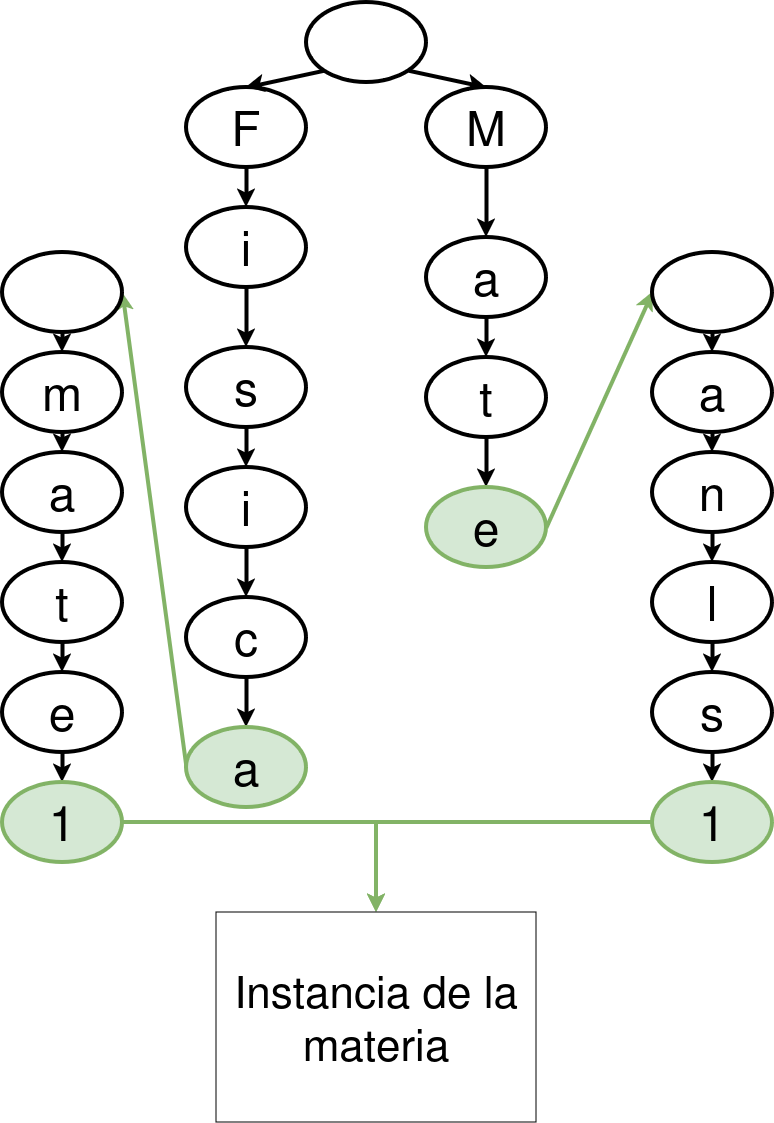
\includegraphics[width=0.5\textwidth]{diagrama1.png}
\end{figure*}
\pagebreak
\section*{Dudas:}
\begin{figure*}[h]
    \centering
    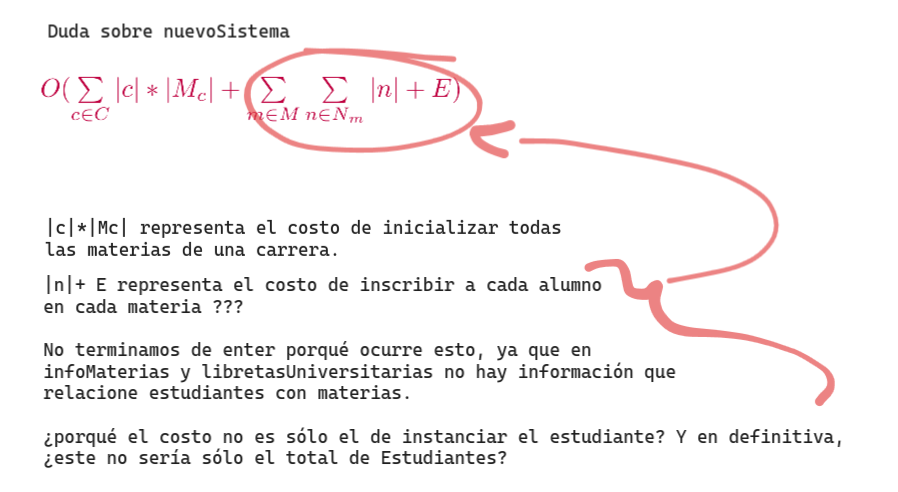
\includegraphics[width=0.7\textwidth]{duda1.png}
\end{figure*}
\pagebreak
\section*{Pseudoresoluciones:}
{\vspace*{-2ex}\hspace*{4em} \small Las que pase a limpio al menos.}


\subsection*{7. carreras(in sistema: SistemaSIU):seq\smm{string}}
\{

\{

    ArrayList lista = new ArrayList() \hfill $\color{Purple}\longleftarrow O(1)$
    
    Iterador it= nuevo iterador del sistemaSIU \hfill $\color{Purple}\longleftarrow O(1)$

    while(iterador.haySiguiente()){\hfill $\color{Purple}\longleftarrow O(\sum_{c\in C}^{} |c|)$

        \hspace*{1.5em} lista.add(iterador.siguiente())

    }

    return lista \hfill $\color{Purple}\longleftarrow O(1)$

\}\hfill $\color{Purple} O(1+1+\sum_{c\in C}^{} |c| +1 )\equiv O(\sum_{c\in C}^{} |c|)$

\noindent\}

\salto{\baselineskip}
\anotacionns[ForestGreen]{Nota: el iterador del trie devuelve los strings ordenador de forma lexicografica.}

\subsection*{8. materias(in sistema: SistemaSIU, in carrera: string):seq\smm{string}}
\{

\{

    Materias materia = Carreras.buscar(carrera) \hfill $\color{Purple}\longleftarrow O(|carrera|)$

    ArrayList lista = new ArrayList() \hfill $\color{Purple}\longleftarrow O(1)$
    
    Iterador it= nuevo iterador del la carrera \hfill $\color{Purple}\longleftarrow O(1)$

    while(iterador.haySiguiente()){\hfill $\color{Purple}\longleftarrow O(\sum_{m_c\in M_c}^{} |m_c|)$

        \hspace*{1.5em} lista.add(iterador.siguiente())

    }

    return lista \hfill $\color{Purple}\longleftarrow O(1)$

\}

\noindent\}\hfill $\color{Purple} O(|carrera|+1+1+\sum_{m_c\in M_c}^{} |m_c| +1 )\equiv O(|carrera|+\sum_{m_c\in M_c}^{} |m_c|)$

\salto{\baselineskip}
\anotacionns[ForestGreen]{Nota: el iterador del trie devuelve los strings ordenador de forma lexicografica.}

\{

    Trie materias = Carreras.buscar(nombreCarrera) \hfill $\color{Purple}\longleftarrow O(|nombreCarrera|)$

    Materia materia =  materias.buscar(nombreMateria) \hfill $\color{Purple}\longleftarrow O(|nombreMateria|)$

    Iterador iteNomMaterias = nuevo iterador materia.listaTuplas \hfill $\color{Purple}\longleftarrow O(1)$
    
    while (iteNomMaterias.haySiguiente())\{\hfill $\color{Purple}\longleftarrow O(\sum_{n\in N_m}^{} |n|)$

    \hspace*{1.5em} tupla\smm{Carrera, String} tuplaInfo = iteNomMaterias.siguiente() \hfill $\color{Purple}\longleftarrow O(1)$

    \hspace*{1.5em} tuplaInfo[0].eliminar(tuplaInfo[1]) \hfill $\color{Purple}\longleftarrow O(|nombreMateria|)$

    \}

    Iterador iteEstudiante = nuevo iterador materia.listaInscriptos\hfill $\color{Purple}\longleftarrow O(1)$

    while (iteEstudiante.haySiguiente())\{\hfill $\color{Purple}\longleftarrow O(E_m)$

    \hspace{1.5em} luActual = iteEstudiante.siguiente() \hfill $\color{Purple}\longleftarrow O(1)$

    \hspace*{1.5em} SistemaSIU.estudiantes.restarUno(luActual) \hfill $\color{Purple}\longleftarrow O(1)$
    
    \}

\}\hfill {$\color{Purple} |nombreCarrera|+|nombreMateria|+\sum_{n\in N_m}^{} |n| + E_m $ \color{Purple}(\emph{o algo asi})}
\pagebreak
\section*{Resumen:}

\salto{\baselineskip}

\begin{design}{Materia}{nada}
    \var{contadorInscriptos}{int}
    \var{listaInscriptos}{ArrayList\smm{String}}
    \var{listaTuplas}{ArrayList\smm{ tupla\smm{Carrera, String} }}
    \var{docentes}{Arreglo<int>[4]}
\end{design}

\begin{design}{SistemaSIU}{nada}
    \var{Carreras}{Trie \smm{Trie\smm{Materia} }}
    \var{Estudiantes}{Trie \smm{int}}

\end{design}
\begin{design}{Trie\smm{B}}{Diccionario\smm{B}}
    
    {\color{ForestGreen} Como implementamos un trie? es el dicicionario sobre trie que vimos en el laboratorio?}
\end{design}

Carreras seria una instancia de Trie cuyos nodos significativos apuntan a otros tries, que representan a las materias.

Materias es una instancia de Trie cuyos nodos significativos son instancias de Materia.

Estudiantes es una instancia de Trie cuyos nodos significativos seran la cantidad de materias a las que este estudiante esta incripto.


\end{document}